\section{Partiella differentialekvationer}

\paragraph{Dirichletvillkor}
Betrakta en differentialekvation som skall lösas på ett domän $\Omega$. Dirichletvillkor är på formen 
\begin{align*}
	u(x, t) = 0, x\in\bound{\Omega}.
\end{align*}

\paragraph{Neumannvillkor}
Betrakta en differentialekvation som skall lösas på ett domän $\Omega$. Neumannvillkor är på formen
\begin{align*}
	n_{i}\del{i}{u(x, t)} = 0, x\in\bound{\Omega},
\end{align*}
där $n$ är normal på $\bound{\Omega}$.

\paragraph{Robinvillkor}
Betrakta en differentialekvation som skall lösas på ett domän $\Omega$. Robinvillkor är på formen
\begin{align*}
	\alpha(x, t)u(x, t) + \beta(x, t)n_{i}\del{i}{u(x, t)} = 0, x\in\bound{\Omega},
\end{align*}
där $n$ är normal på $\bound{\Omega}$.

\paragraph{Homogena och inhomogena grejer}
En differentialekvation på formen
\begin{align*}
	Lu = f
\end{align*}
kallas för homogen om $f = 0$ och inhomogen annars. Vi definierar homogena och inhomogena randvillkor analogt.

\paragraph{Flerdimensionell variant av Sturm-Liouvilles sats}
Problemet
\begin{align*}
	&\laplace{f} = \lambda f, \\
	&f(x) = 0, x\in\bound{\Omega}
\end{align*}
har oändligt många lösningar $f_{n}$ med distinkta egenvärden $\lambda_{n} > 0$ så att lösningarna är ortogonala med inreprodukten
\begin{align*}
	\inprod{f}{g} = \integ[n]{\Omega}{x}{\cc{f}(x)g(x)}.
\end{align*}

För problemet
\begin{align*}
	&\laplace{f} = \lambda f, \\
	&\alpha(x, t)u(x, t) + \beta(x, t)n_{i}\del{i}{u(x, t)} = 0, x\in\bound{\Omega},
\end{align*}
där $n$ är normal på $\bound{\Omega}$, finns det oändligt många ortogonala lösningar med distinkta egenvärden.

\paragraph{Lösning av PDE:er for dummies}
\begin{figure}[!ht]
	\centering
	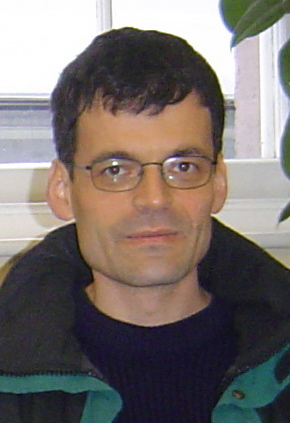
\includegraphics[width = 0.2\textwidth]{./Images/langmann.jpg}
	\caption{Peak fysiker.}
	\label{fig:langmann}
\end{figure}
Fysiker hatar honom. Här kan du läsa hans tre enkla steg för att göra teoretisk fysik komplett vid att lösa partiella differentialekvationer:
\begin{enumerate}
	\item Bestäm lösningar till det homogena problemet.
	\item Välj lösningar som passar till randvillkoren. Sturm-Liouvilles sats garanterar att det finns lösningar. Låt den allmänna lösningen vara en linjärkombination av dessa.
	\item Hitta motsvarande lösningar till variabler som inte har randvillkor.
	\item Skriv upp den allmänna lösningen som en linjärkombination av lösningarna du har fått innan.
	\item Välj koefficienter som passar till initialvillkoren. Det finns även satser som hjälper med detta.
\end{enumerate}

\paragraph{Separationsmetoden}
Separationsmetoden är ett sätt att lösa homogena partiella differentialekvationer på.

Låt $u(x_{1}, \dots, x_{n})$ vara en lösning till $Lu = 0$, där $L$ är en linjär differentialoperator. Separationsmetoden går ut på att göra ansatsen
\begin{align*}
	u = \prod\limits_{i = 1}^{n}X_{i}(x_{i}).
\end{align*}
Denna ansatsen gör förhoppningsvis att differentialekvationen kan skrivas som
\begin{align*}
	\frac{1}{X_{1}}L_{1}X_{1} = \frac{1}{\prod\limits_{i = 1}^{n}X_{i}}L'\prod\limits_{i = 1}^{n}X_{i}.
\end{align*}
Varje sida beror av olika variabler, varför de måste vara lika med en konstant. På detta sättet kan det ursprungliga problemet förhoppningsvis separeras i delproblem som är enkla att lösa.